
\chapter{Information Visualization}
\label{chap:InfoVis}

Information visualization seeks to use interactive graphics to assist
in the analysis and presentation of abstract information. Information
visualization builds on capabilities of human visual perception,
including the rapid scanning, recognition, and recall of visual
information, as well as the automatic detection of visual patterns. In
contrast to textual representations of data, the processing of
well-designed visualizations requires less cognitive effort,
because it leverages features of the human visual processing
system. One of these features is \emph{preattentive processing},
whereby certain visual attributes can be processed very quickly and
without conscious effort \parencite{PreattentiveProcessing}.
% KA give an example of a pre-attentive feature


In addition to visuals being easier to assimilate by humans, a purely
textual and statistical view of data can also lead to erroneous
assumptions. This is demonstrated in Anscombe's famous example of four
completely different datasets (variables in $x$ and $y$) having
identical summary statistics (mean and standard deviation), called
Anscombe's Quartet \parencite{AnscombesQuartet}, shown in
Table~\ref{tab:AnscombeTable}. An observer trying to understand these
datasets from their summary statistics alone might mistakenly deem
them to be identical. Their inequality only becomes obvious after
carefully examining and comparing the individual entries in the
datasets themselves.
%
However, the differences in the four datasets are immediately obvious
when plotted graphically, as can be seen in
Figure~\ref{fig:AnscombePlot}. Even though Anscombe's Quartet is
likely the most famous example demonstrating this characteristic, it
is certainly not the only example, as has been shown by
\textcite{GenDataIdenticalStatisticsDissimilarGraphics}.



\begin{table}[tp]
\centering
\tablestretch
\rowcolors{3}{tablerowcolour}{}
\begin{small}
\begin{tabular}{>{\kern-\tabcolsep}rcrrcrrcrrcrr<{\kern-\tabcolsep}}
\toprule
\hiderowcolors
  & \phantom{i} &
  \multicolumn{2}{c}{$\mathbf{v_1}$} & \phantom{a} &
  \multicolumn{2}{c}{$\mathbf{v_2}$} & \phantom{a} &
  \multicolumn{2}{c}{$\mathbf{v_3}$} & \phantom{a} &
  \multicolumn{2}{c}{$\mathbf{v_4}$} \\
\cmidrule(l{1em}r){3-4}\cmidrule(l{1em}r){6-7}\cmidrule(l{1em}r){9-10}\cmidrule(l{1em}r){12-13}
  & & $x_1$ &  $y_1$ & &  $x_2$ & $y_2$ & & $x_3$ &  $y_3$ & &  $x_4$ &  $y_4$ \\
\midrule
\showrowcolors
  & & 10.00 &   8.04 & &  10.00 &  9.14 & &  10.00 &   7.46 & &   8.00 &   6.58 \\
  & &  8.00 &   6.95 & &   8.00 &  8.14 & &   8.00 &   6.77 & &   8.00 &   5.76 \\
  & & 13.00 &   7.58 & &  13.00 &  8.74 & &  13.00 &  12.74 & &   8.00 &   7.71 \\
  & &  9.00 &   8.81 & &   9.00 &  8.77 & &   9.00 &   7.11 & &   8.00 &   8.84 \\
  & & 11.00 &   8.33 & &  11.00 &  9.26 & &  11.00 &   7.81 & &   8.00 &   8.47 \\
  & & 14.00 &   9.96 & &  14.00 &  8.10 & &  14.00 &   8.84 & &   8.00 &   7.04 \\
  & &  6.00 &   7.24 & &   6.00 &  6.13 & &   6.00 &   6.08 & &   8.00 &   5.25 \\
  & &  4.00 &   4.26 & &   4.00 &  3.10 & &   4.00 &   5.39 & &  19.00 &  12.50 \\
  & & 12.00 &  10.84 & &  12.00 &  9.13 & &  12.00 &   8.15 & &   8.00 &   5.56 \\
  & &  7.00 &   4.82 & &   7.00 &  7.26 & &   7.00 &   6.42 & &   8.00 &   7.91 \\
  & &  5.00 &   5.68 & &   5.00 &  4.74 & &   5.00 &   5.73 & &   8.00 &   6.89 \\
\hiderowcolors
\addlinespace[0.5em]
\textbf{mean} & &
  \textbf{9.00} & \textbf{7.50} & &
  \textbf{9.00} & \textbf{7.50} & &
  \textbf{9.00} & \textbf{7.50} & &
  \textbf{9.00} & \textbf{7.50} \\
\textbf{sd} & &
  \textbf{3.3166} & \textbf{2.0316} & &
  \textbf{3.3166} & \textbf{2.0317} & &
  \textbf{3.3166} & \textbf{2.0304} & &
  \textbf{3.3166} & \textbf{2.0306} \\
\bottomrule
\end{tabular}
\end{small}

\caption[Anscombe's Quartet in Tabular Form]
{
The four datasets (variables) in Anscombe's Quartet look identical if
only standard summary statistics like mean and standard deviation are
considered. The difference between the datasets is only apparent after
careful examination of the numbers.
}
\label{tab:AnscombeTable}
\end{table}



\begin{figure}[tp]
\centering
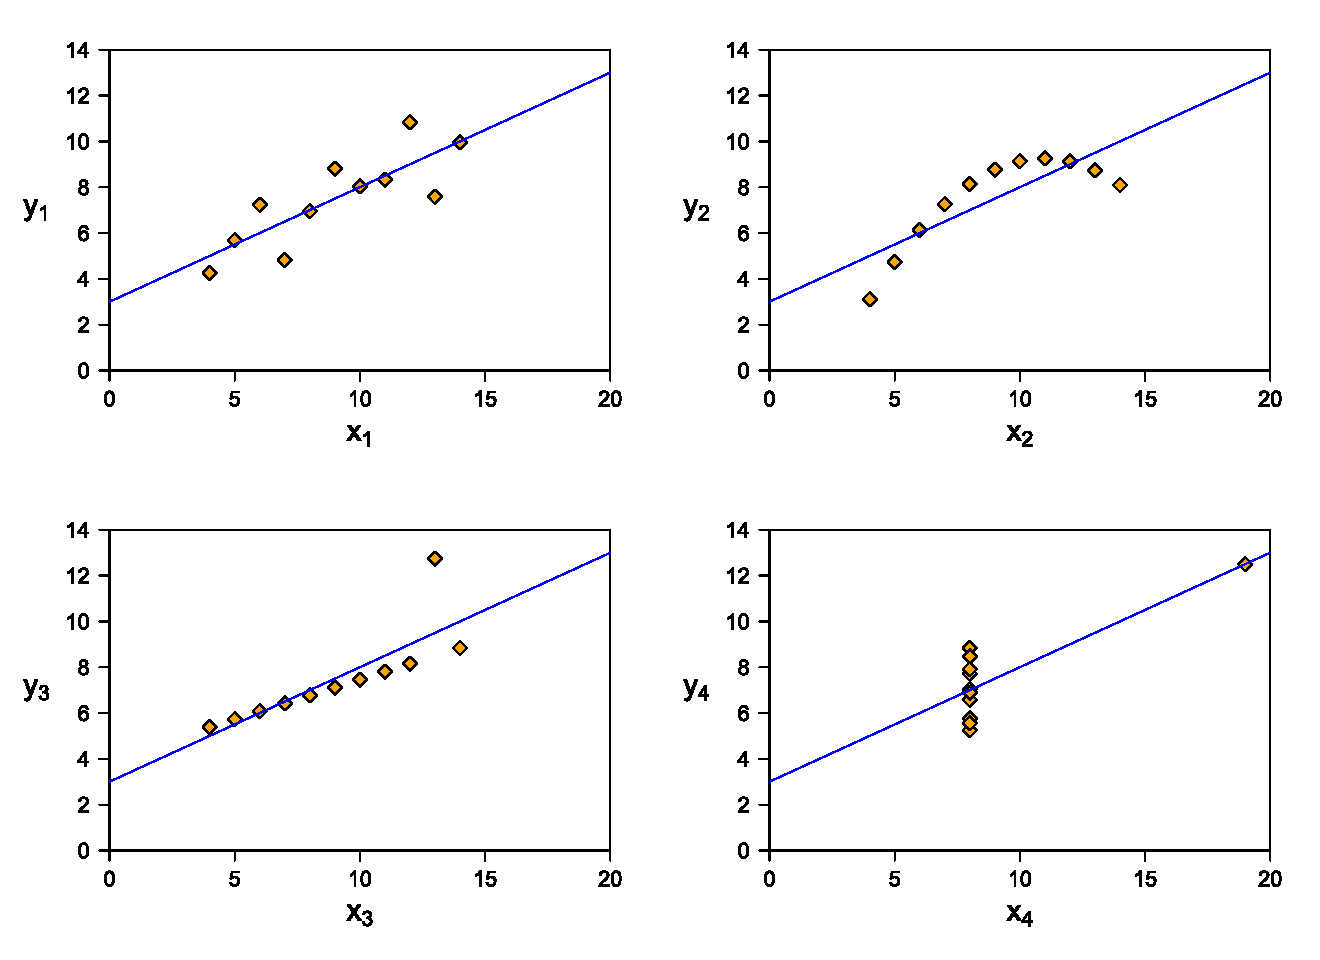
\includegraphics[keepaspectratio,width=\linewidth,height=\halfh]
{diagrams/anscombe.pdf}
\caption[Anscombe's Quartet]{
When plotted graphically, it is immediately apparent that
the four datasets in Anscombe's Quartet are very different.
\imgcredit{Image extracted from \textcite{IVISCourseNotes}.
Used with kind permission by Keith Andrews.}
}
\label{fig:AnscombePlot}
\end{figure}







This thesis adheres to the characterization of the field of
visualization as having three main subfields, as defined by
\textcite{IVISCourseNotes}:
\begin{enumerate}
\item \liintro{Information Visualization (InfoVis)}: Deals with
  abstract data, which has no inherent geometry or visual form and for
  which a suitable type of visualization has to be chosen.

\item \liintro{Geographic Visualization (GeoVis)}: Deals with
  map-based data which has inherent 2d or 3d spatial geometry.

\item \liintro{Scientific Visualization (SciVis)}: Deals with
  real-world objects having inherent 2d or 3d geometry, which
  is used as the basis for visualization.
\end{enumerate}
The often-used term \enquote{data visualization} (\emph{DataVis}) is
defined as the combination (union) of information visualization and
geographic visualization.


Visualizations presented in an interactive medium do not merely
consist of visual representations. It is equally important to provide
means for interacting with these representations to analyze more
complex datasets. Without interactions, a visualization is just a
static image and has only very limited use when dealing with large and
multidimensional datasets. Even though the majority of attention in
the field of information visualization has been directed towards the
presentational aspect of visualizations, research has also been done
on their interactive aspects. Numerous taxonomies have been formulated
with the goal of defining the design space of interactions to support
analytic reasoning, but they vary greatly depending on the concepts
they are focusing on. Some taxonomies have been defined on the concept
of low-level interaction techniques
\parencite{TheEyesHaveIt,GrammarOfGraphics}, providing a very
system-centric view on interaction. Other taxonomies focus on user
tasks \parencite{LowLevelComponentsOfAnalyticActivity}, which are not
necessarily strongly related to interacting with visualizations.
\textcite{RoleOfInteractionInInformationVisualization} aims to provide
a view in between the purely system-centric and purely user-centric
extremes by defining a taxonomy based on what a user wants to achieve,
also known as \emph{user intent}. The categories of this taxonomy are
shown in Table~\ref{tab:UserIntentCategories}. They provide a good
framework for the discussion of interactivity in the context of
information visualization.


\begin{table}[tp]
\tablestretch
\rowcolors{2}{}{tablerowcolour}
\centering
\begin{small}
\begin{tabularx}{\linewidth}{>{\kern-\tabcolsep}lL{0.35\linewidth}X<{\kern-\tabcolsep}}
\toprule
Category & Description & Examples \\
\midrule
Select &
  Mark something as interesting. &
  Highlighted selections, placemarks, assigning classes. \\
Explore &
  Show me something else. &
  Different subset of data, panning, direct-walk. \\
Reconfigure &
  Show me a different arrangement. &
  Sorting, rearranging columns, plotting different dimensions, using an alternative projection. \\
Encode &
  Show me a different representation. &
  Changing visual encoding (color, size, shape), or even chart type. \\
Abstract / Elaborate &
  Show me more or less detail. &
  Details-on-demand, drill-down and roll-up, tooltips, zooming in and out. \\
Filter &
  Show me something conditionally. &
  Dynamic queries, range sliders, toggle buttons, query by example. \\
Connect &
  Show me related items. &
  Brushing across views, highlighting connected items on mouseover. \\
\bottomrule
\end{tabularx}
\end{small}
\caption[Categories of Interaction Based on User Intent]{
Categories of interaction with visualizations based on what
a user wants to achieve (user intent).
\imgcredit{From \textcite{RoleOfInteractionInInformationVisualization}}
}
\label{tab:UserIntentCategories}
\end{table}






\section{History of Information Visualization}

The history of information visualization goes back a long time. One of
its earliest examples dates back to the \nth{10} Century, when an
unknown astronomer created the chart about the movement of prominent
planets \parencite{CommentariiInSomniumScipionis} shown in
Figure~\ref{fig:PlanetaryMovements}.
% KA: 1175 is the 12th Century not the 10th
Other noteworthy early visualizations include the first occurrence of
the principle which \textcite{VisualDisplayOfQuantitativeInformation}
later called \enquote{small multiples} in the 1626 chart by
\textcite{RosaUrsina} demonstrating sunspot changes shown in
Figure~\ref{fig:SunspotChanges}, and the 1644 chart displaying
longitudinal distance determinations between Toledo and Rome by \textcite{RomeToledoBook} shown in
Figure~\ref{fig:RomeToledoLongitude}.


\begin{figure}[tp]
\centering
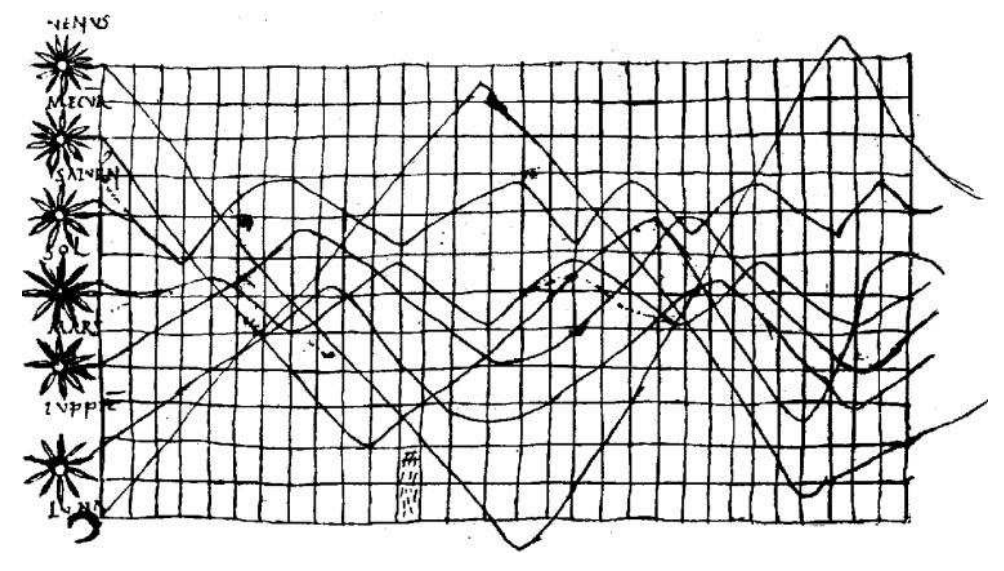
\includegraphics[keepaspectratio,width=\linewidth,height=\thirdh]
{images/planetary-movements.png}
\caption[Chart of Planetary Movements from the \nth{10} Century]{%
A line chart created by an unknown astronomer in the \nth{10} Century,
depicting the movements of seven prominent planets.
\imgcredit{Image extracted from \textcite{BriefHistoryOfDataVis}.
Original appearance in \textcite{CommentariiInSomniumScipionis}.}
}
\label{fig:PlanetaryMovements}
\end{figure}
% KA Original appearance in Macrobius [1175] ??
% Funkhouser 1936 says 10th or 11th Century



\begin{figure}[tp]
\centering
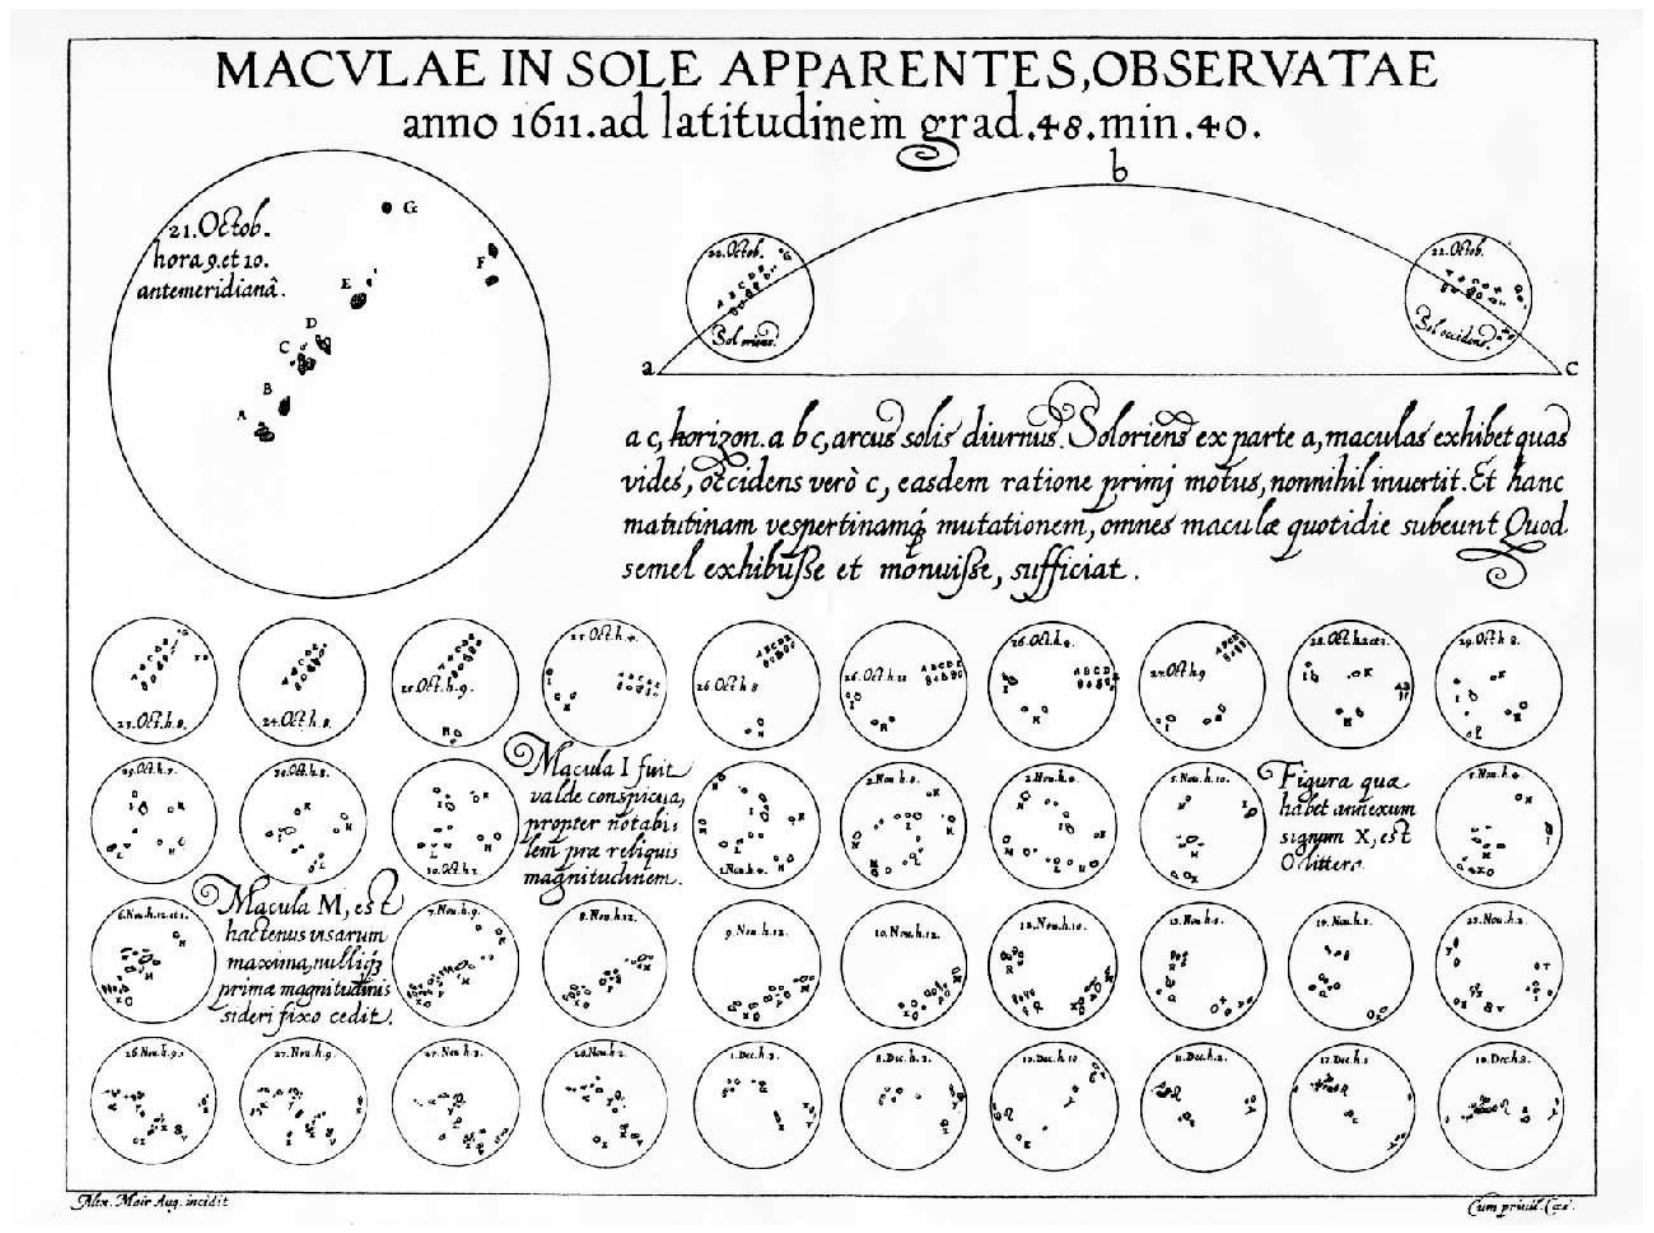
\includegraphics[keepaspectratio,width=\linewidth,height=\thirdh]
{images/sunspot-changes.png}
\caption[Chart of Changes in Sunspots from 1626]{%
The observed changes in sunspots based on recordings
of two months of data from 1611. It is the first occurrence of the
principle later called \enquote{small multiples} by
\textcite{VisualDisplayOfQuantitativeInformation}.
\imgcredit{Image extracted from \textcite{BriefHistoryOfDataVis}.
Original appearance in \textcite{RosaUrsina}.}
}
\label{fig:SunspotChanges}
\end{figure}

% https://cudl.lib.cam.ac.uk/view/PR-QQ-AST-00002-00158-B-00003/1

% Tufte, Edward R. and Peter R. Graves-Morris [1983].
% The Visual Display of Quantitative Information.
% Graphics Press, 1983. ISBN 1930824130 (cited on pages 19–20).
% KA: who is Graves-Morris ?



\begin{figure}[tp]
\centering
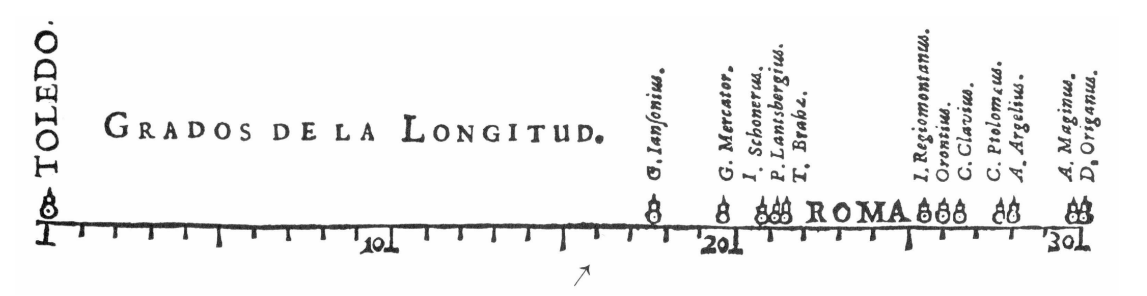
\includegraphics[keepaspectratio,width=\linewidth,height=\thirdh]
{images/rome-toledo-longitude.png}
\caption[Chart of Longitudinal Distance Determinations Between Toledo and Rome From 1644]{%
A comparison of the twelve known estimates in longitudinal
distance between Rome and Toledo by various astronomers. The correct
distance is marked by the arrow beneath. It is considered by \textcite[15]{VisualExplanations} to be the
first visual representation of statistical data.
\imgcredit{Image extracted from \textcite{BriefHistoryOfDataVis}.
Original appearance in \textcite{RomeToledoBook}.}
}
\label{fig:RomeToledoLongitude}
\end{figure}





William Playfair (1759--1823) is considered by many to be one of the
forefathers of modern information visualization. His published works
contain the first occurrences of many graphical forms still widely
used today. In one of his earlier works
\parencite{CommercialAndPoliticalAtlas}, he introduced the concepts of
line charts (Figure~\ref{fig:PlayfairLineChart}), bar charts
(Figure~\ref{fig:PlayfairBarChart}), and area charts
(Figure~\ref{fig:PlayfairAreaChart}) to communicate economic factors
of England during the eighteenth century. In a related later work
\parencite{StatisticalBreviary}, he used the first ever published pie
and circle charts to show and compare the resources of states and
kingdoms in Europe. The charts he created are very similar to modern
ones, containing familiar concepts such as labeled axes, grids,
titles, and color-coding.



\begin{figure}[tp]
\centering
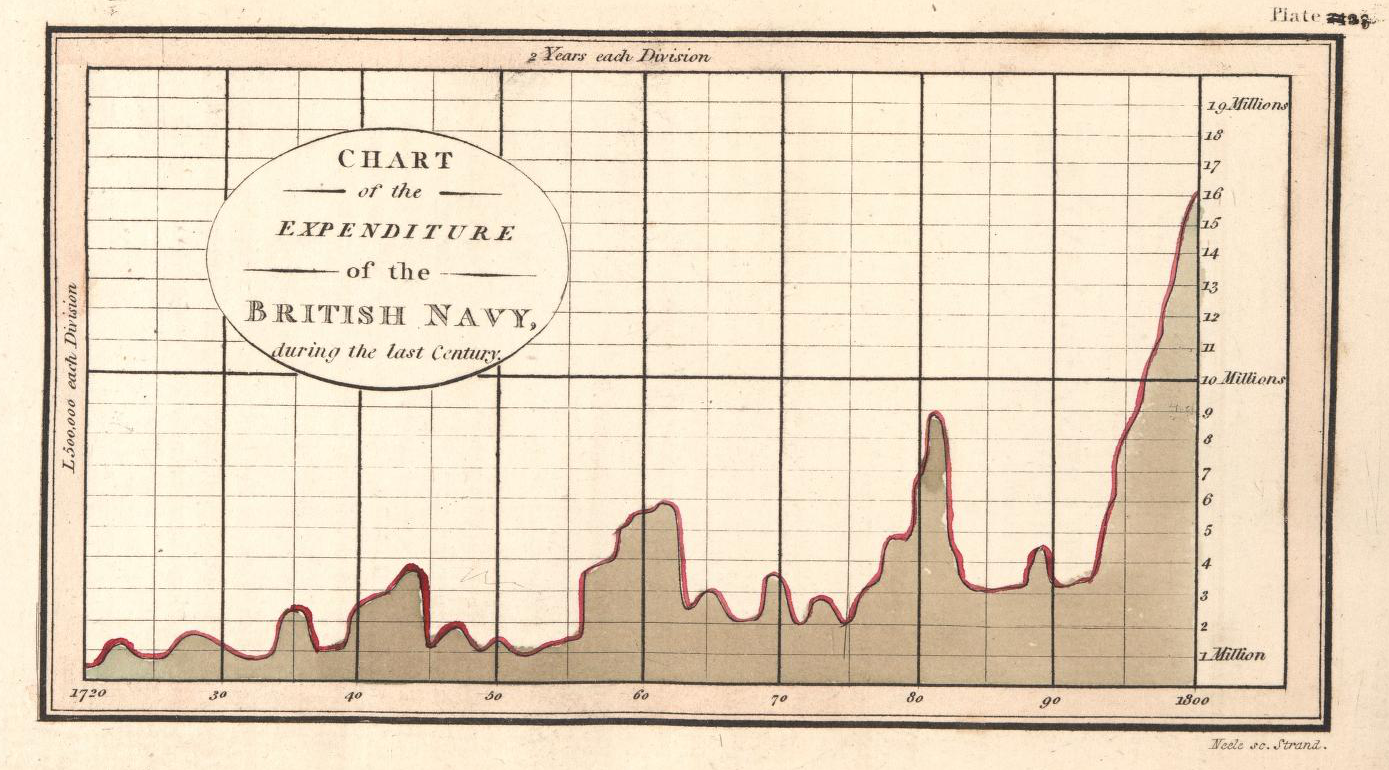
\includegraphics[keepaspectratio,width=\linewidth,height=\thirdh]
{images/playfair-line-chart.png}
\caption[Line Chart by William Playfair from 1786]{%
Line chart of the expenditure of the British Navy during the \nth{18}
Century. It was published in 1786 and is considered to be one of the
first occurrences of a line chart containing components found in
modern visualizations.
\imgcredit{Image extracted from Schoenberg Center for
Electronic Text and Image (SCETI).
Used under the terms of Creative Commons CC BY 2.5.}
}
\label{fig:PlayfairLineChart}
\end{figure}



\begin{figure}[tp]
\centering
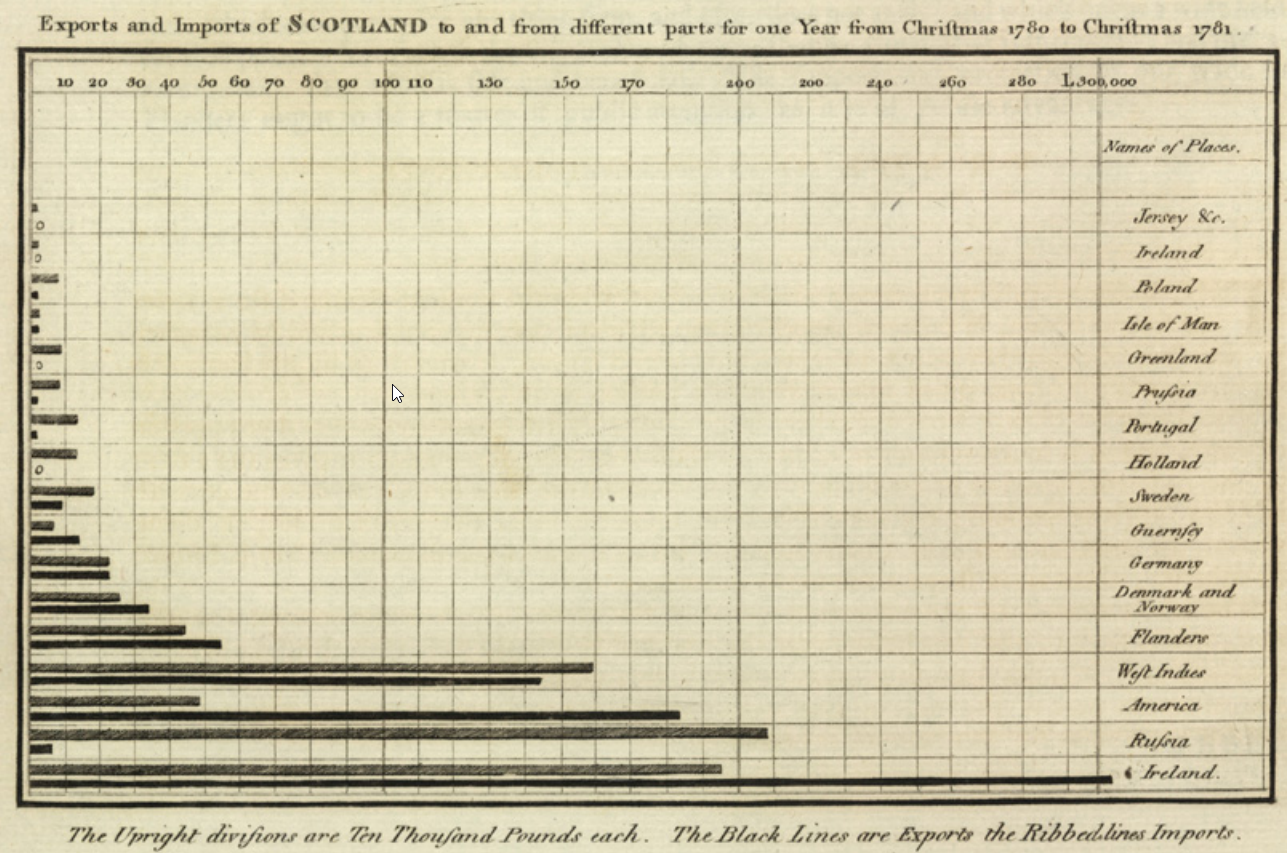
\includegraphics[keepaspectratio,width=\linewidth,height=\thirdh]
{images/playfair-bar-chart.png}
\caption[Bar Chart by William Playfair from 1786]{%
Bar chart of England's exports and imports to and from Scotland in
1781. Published in 1786, it is considered to be one of the
first occurrences of a bar chart containing most components found in
modern visualizations.
\imgcredit{Image extracted from Schoenberg Center
for Electronic Text and Image (SCETI).
Used under the terms of Creative Commons CC BY 2.5.}
}
\label{fig:PlayfairBarChart}
\end{figure}



\begin{figure}[tp]
\centering
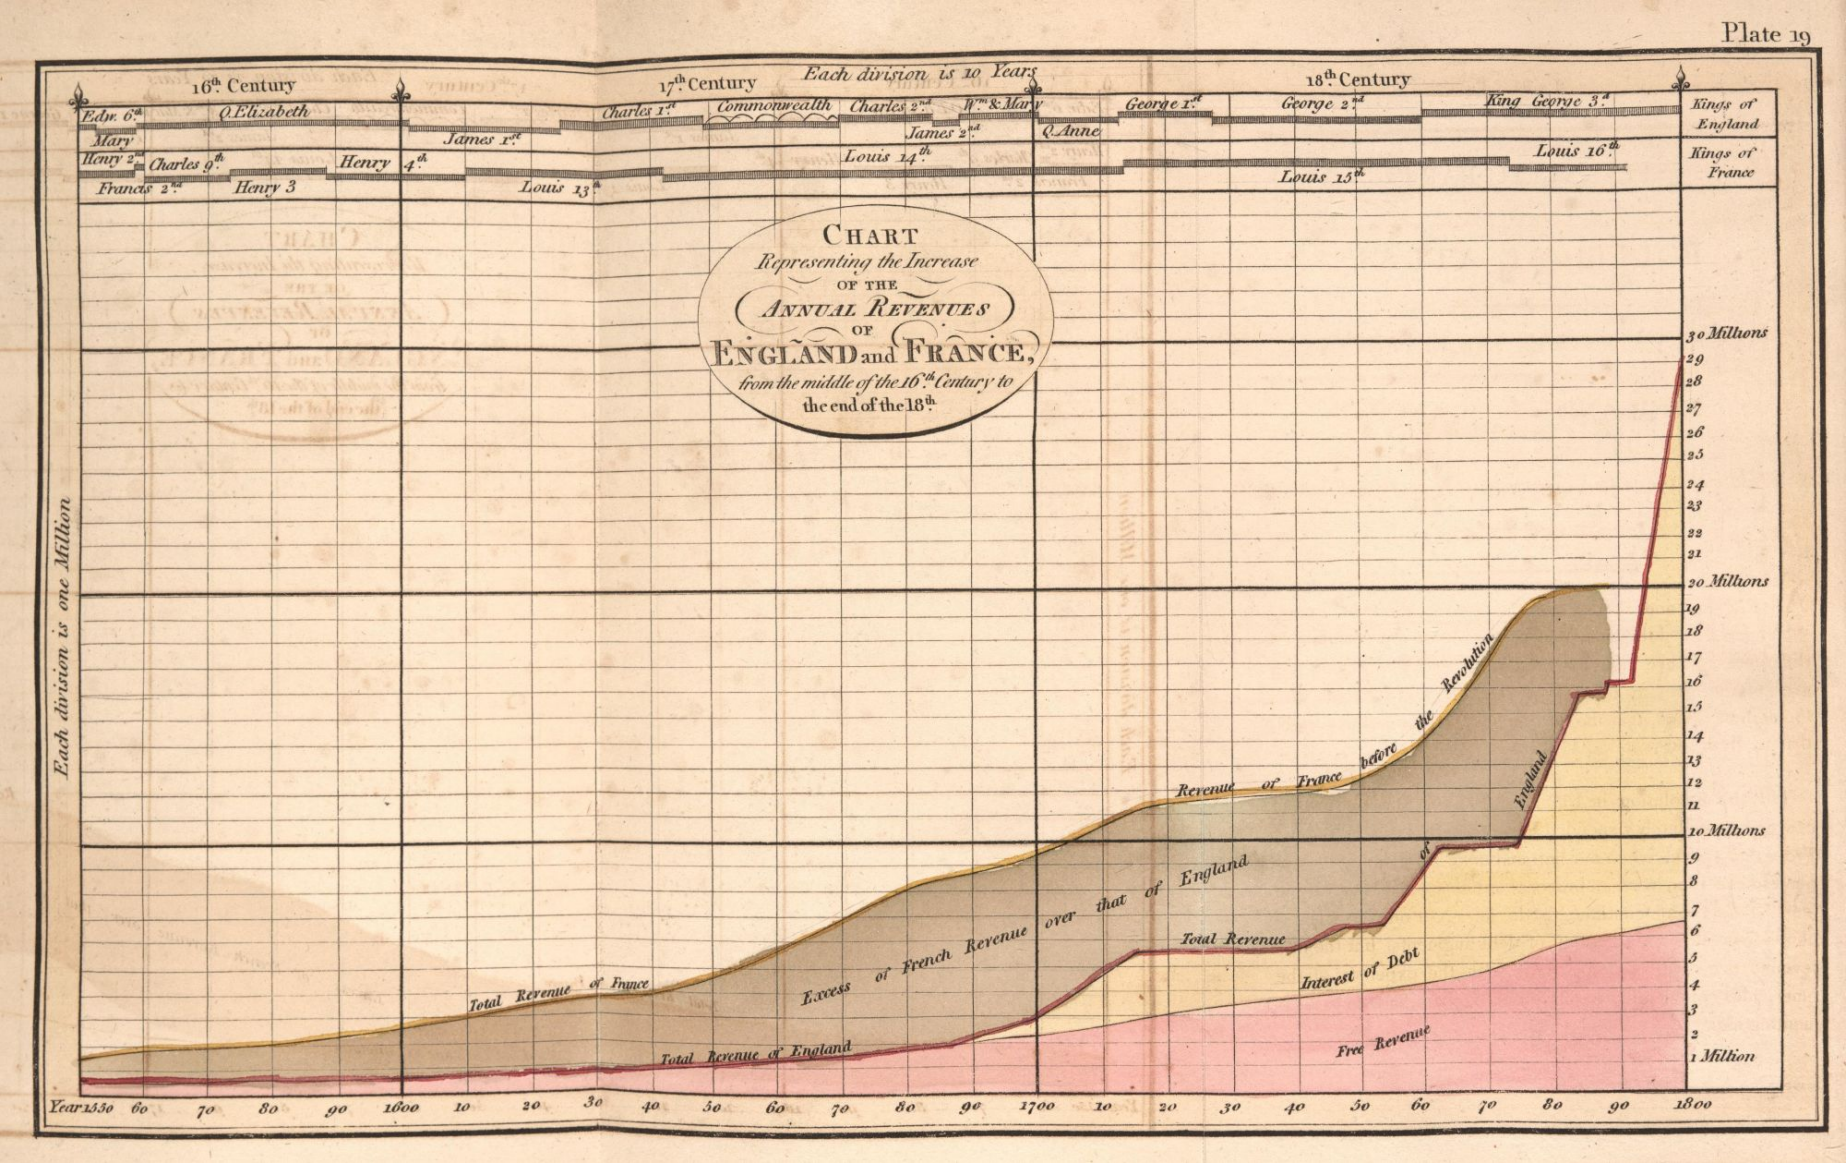
\includegraphics[keepaspectratio,width=\linewidth,height=\thirdh]
{images/playfair-area-chart.png}
\caption[Area Chart by William Playfair from 1786]{%
Area chart of annual revenues of England and France between
1550 and 1800. Published in 1786, it is considered to be one of
the first occurrences of an area chart
containing most components found in modern visualizations.
\imgcredit{Image extracted from Schoenberg Center
for Electronic Text and Image (SCETI).
Used under the terms of Creative Commons CC BY 2.5.}
}
\label{fig:PlayfairAreaChart}
\end{figure}




%% The dot map created by \textcite{ModeOfCommunicationOfCholera} in 1855
%% to trace cholera outbreaks in London (Figure~\ref{fig:CholeraDotMap})
%% is undoubtedly one of the most famous and influential visualizations
%% in history.  Even though it is not directly an information
%% visualization but rather a geographic one, it has been included here
%% because of its historic relevance.  This iconic dot map was used to
%% identify a cluster of cholera-related deaths near a contaminated water
%% pump on Broad Street, leading to the recognition of cholera as a
%% waterborne disease.
%% 
%% 
%% \begin{figure}[tp]
%% \centering
%% 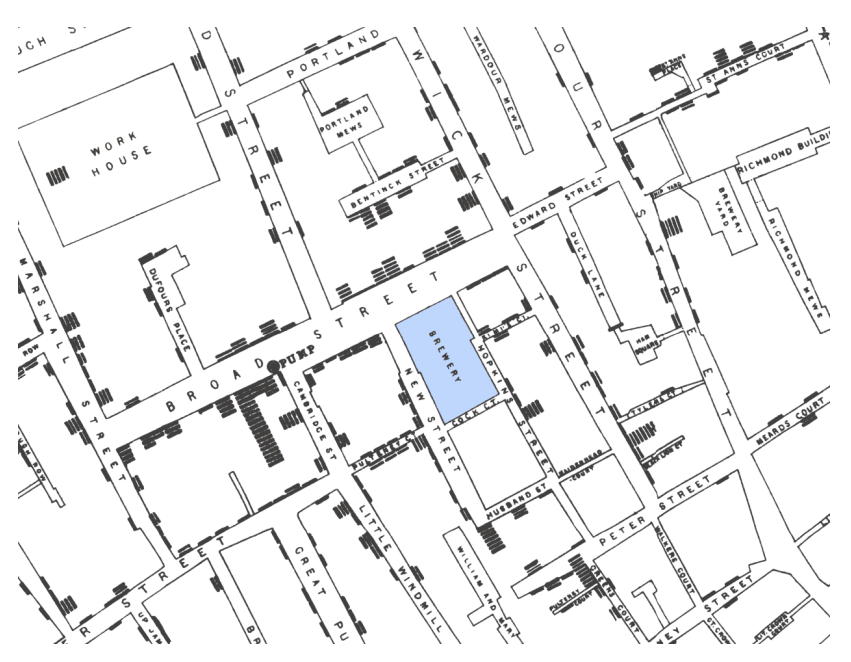
\includegraphics[keepaspectratio,width=\linewidth,height=\fullh / 3]{images/cholera-dot-map.png}
%% \caption[Dot Map Plotting Cholera Deaths in London From 1855]{%
%% This iconic chart was created by Dr. John Snow in 1855 to identify a
%% clustering of cholera-related deaths near Broad Street in London.  It
%% was used to identify a contaminated water pump and to illustrate the
%% waterborne nature of the disease.  Since the data is map-based, this
%% chart is an example of a geographic visualization rather than an
%% information visualization.
%% \imgcredit{Image extracted from \textcite{IVISCourseNotes}.
%% Original appearance in \textcite{ModeOfCommunicationOfCholera}.}
%% }
%% \label{fig:CholeraDotMap}
%% \end{figure}






It would be amiss not to mention Florence Nightingale (1820--1910)
\parencite{FlorenceNightingale} when talking about the history of
information visualization. She was a British statistician, social
reformer, and the founder of modern nursing and might be the first
person who used visualizations to persuade others of a need for
change. During her service as a superintendent of nurses in the
Crimean War, she realized that a large number of deaths in hospitals
resulted from preventable diseases which originated in poor sanitary
conditions. One of her contributions to the field of information
visualization was the creation of a new type of diagram, called a rose
diagram or polar-area chart, shown in
Figure~\ref{fig:NightingalePolarAreaChart}. She used these charts to
communicate data she collected on the mortality of soldiers during the
war and to grab the attention of politicians and the public.

\begin{figure}[tp]
\centering
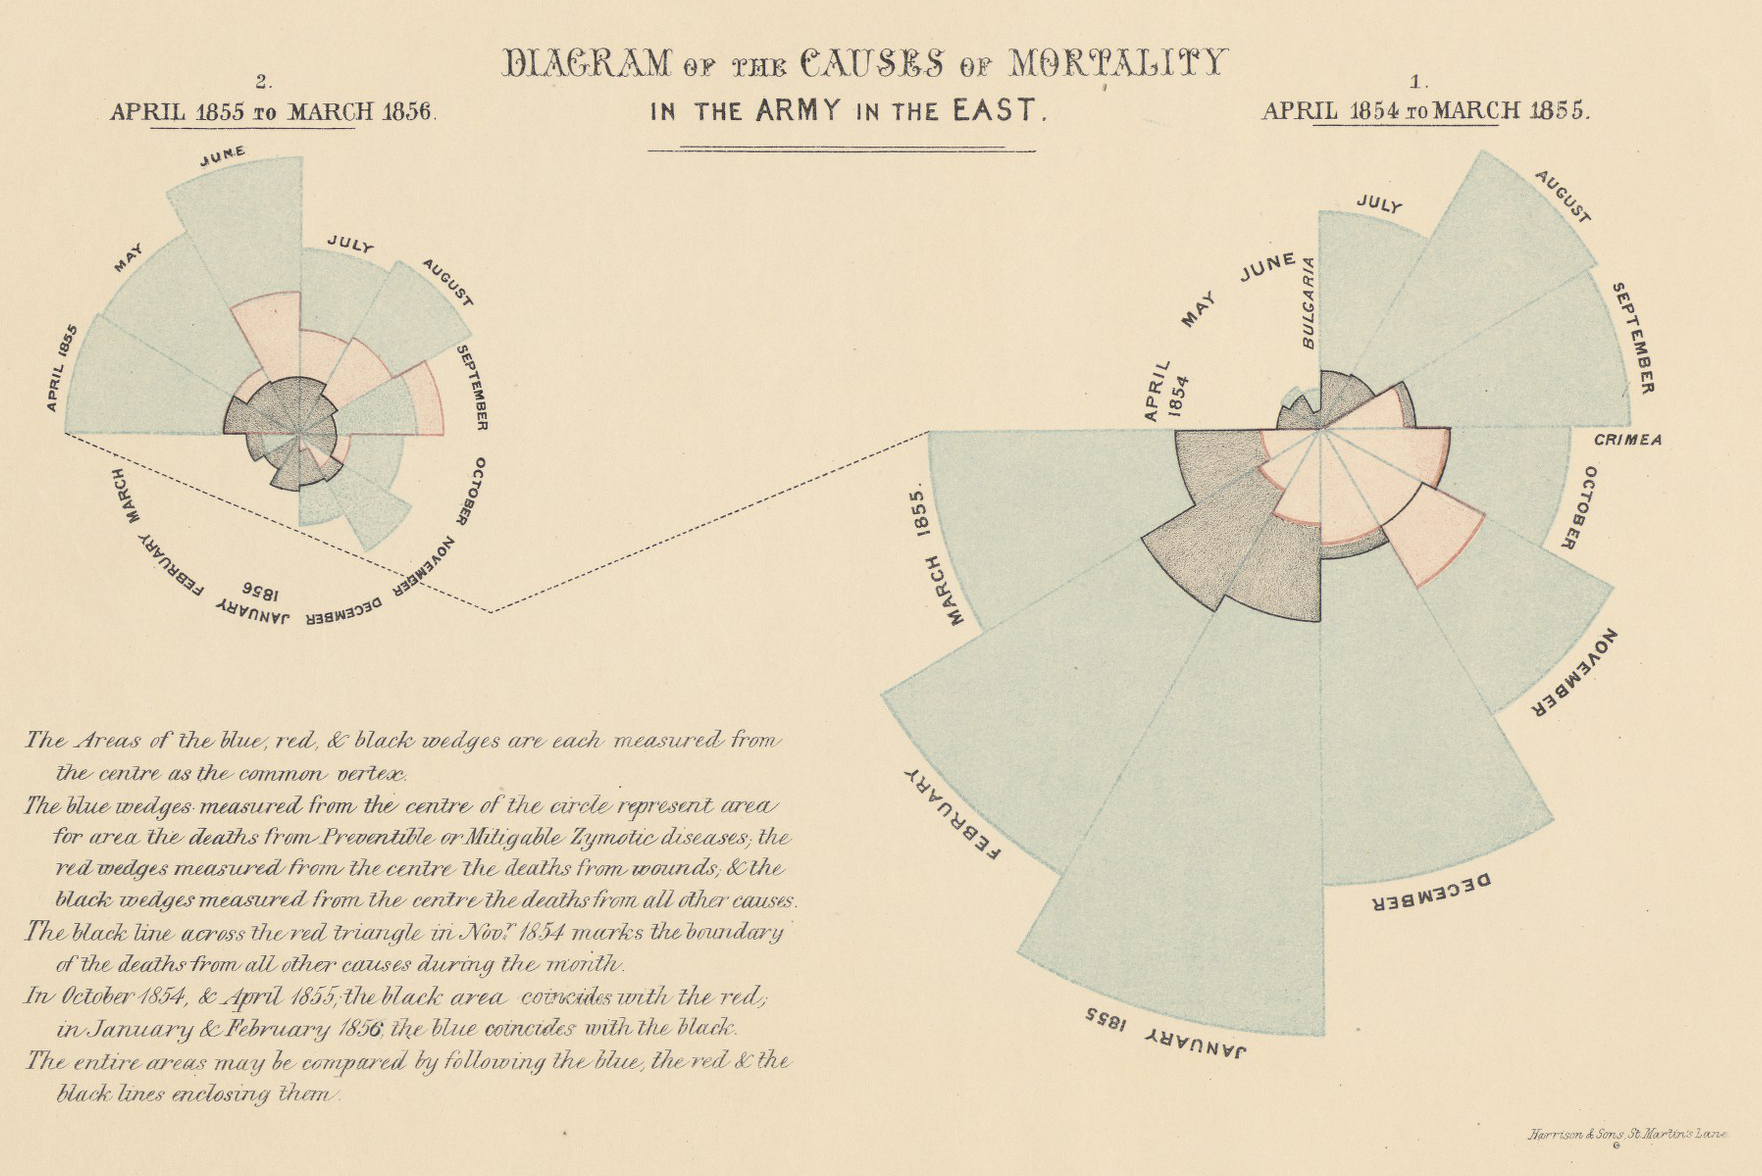
\includegraphics[keepaspectratio,width=\linewidth,height=\thirdh]
{images/nightingale.png}
\caption[Polar-Area Chart by Florence Nightingale from 1859]{%
One of the polar-area charts created by Florence Nightingale in 1859
to convince people of a need for more sanitary conditions in
hospitals. It visualizes the causes of mortality for soldiers during
the Crimean War and demonstrates that a large percentage of patients
died from preventable diseases linked to unsanitary environments.
\imgcredit{Image extracted from Harvard Library.
Used under the terms of Creative Commons Attribution 4.0.}
}
\label{fig:NightingalePolarAreaChart}
\end{figure}




Modern visualizations benefit from the interactive nature of the
devices used to consume them. They can be more complex than static
visualizations, because various interaction techniques enable users to
navigate large amounts of data and make sense of it. High-D by
Macrofocus \parencite{HighD} is a representative example of a modern
interactive visual analytics tool, and is shown in
Figure~\ref{fig:HighD}.

\begin{figure}[tp]
\centering
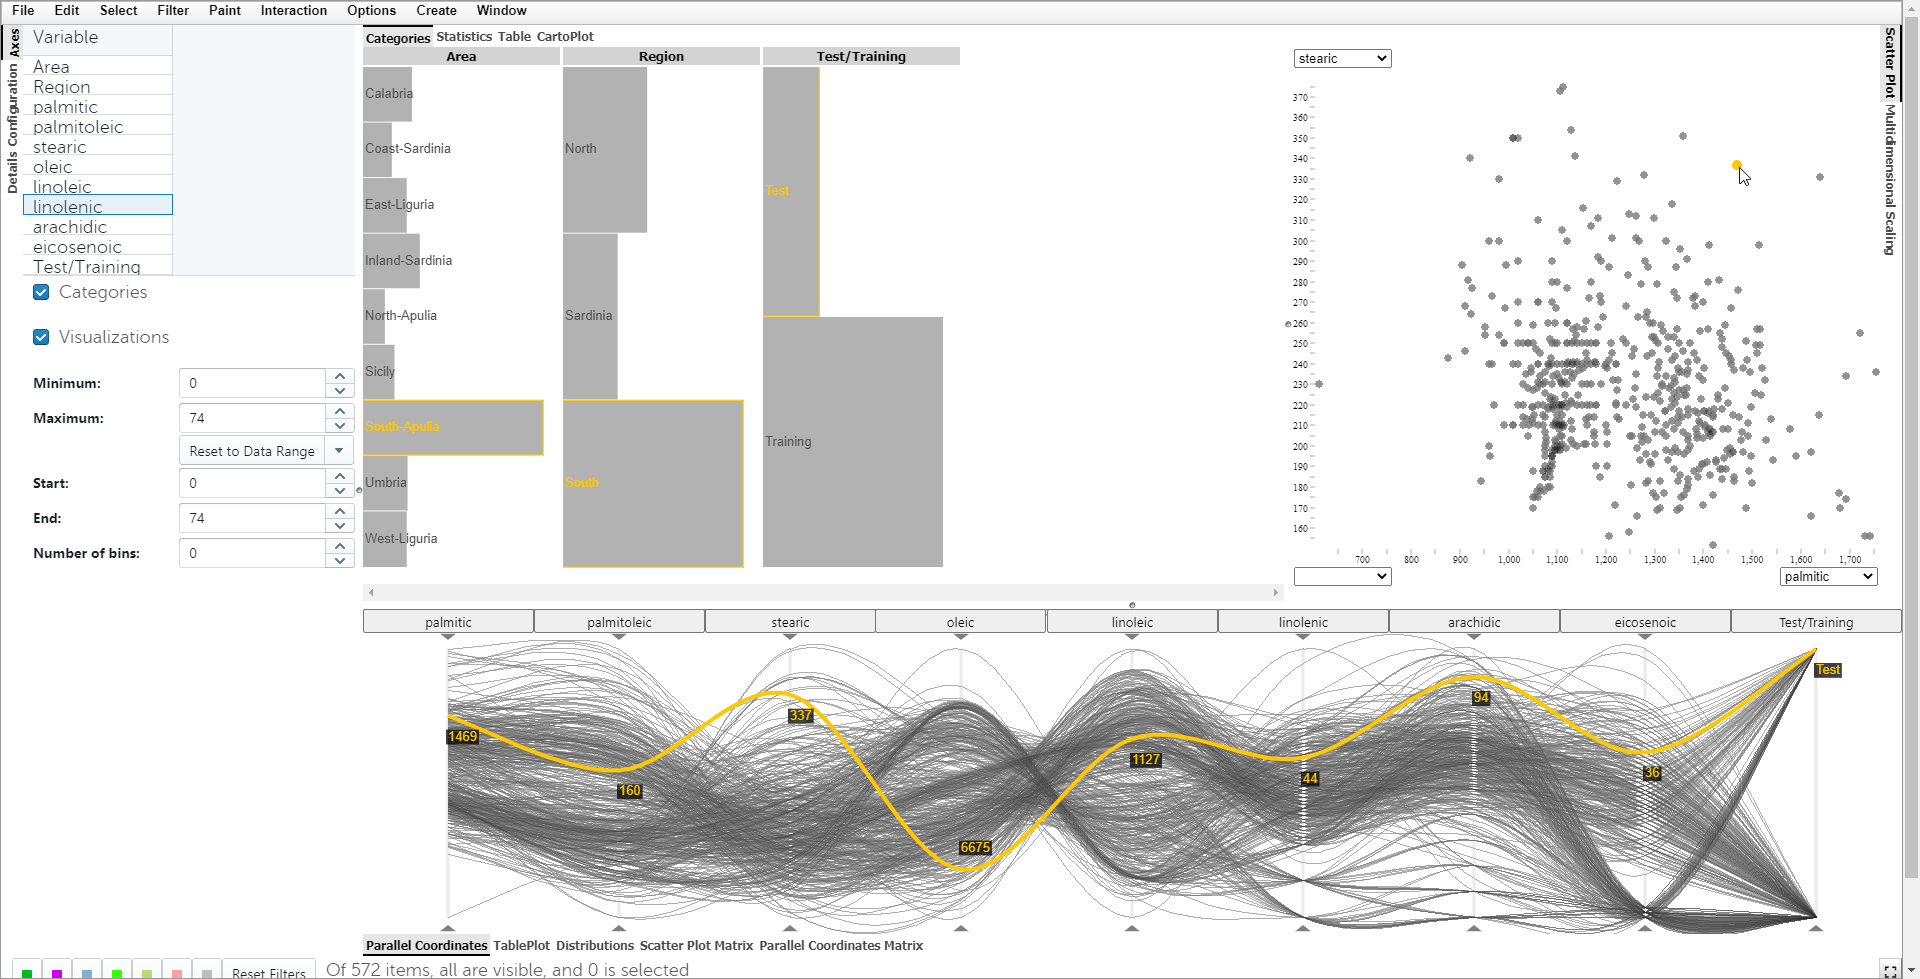
\includegraphics[keepaspectratio,width=\linewidth,height=\thirdh]
{images/high-d.png}
\caption[High-D]{
High-D by Macrofocus is a visual analytics tool
specialized in analyzing multidimensional data.
\imgcredit{Screenshot of High-D \parencite{HighD} taken by the author of this work.}
}
\label{fig:HighD}
\end{figure}




It is out of the scope of this work to provide a full account of the
long and eventful history of information visualization. This section
only provides a brief and very selective view of the topic.  More
comprehensive works for further reading include
\textcite{BriefHistoryOfDataVis}, \textcite{Meirelles-2013},
\textcite{HistoryOfInformationGraphics}, and
\textcite{HistoryOfDataVisAndGraphicCommunication}.










\section{Information Visualization Libraries for the Web}

There are many web-based libraries which simplify the rendering of
interactive visualizations. The approaches used to create and update a
visualization differ widely between libraries. D3 is a low-level
library which enables data-driven transformations of documents. Vega
and Vega-Lite provide a declarative grammar to express the visual and
interactive characteristics of a visualization. Template-based
visualization libraries provide a higher-level template-based
interface which can easily be configured.



\subsection{Data-Driven Documents (D3)}

D3 \parencite{D3} is a free, open-source document manipulation library
built in JavaScript by Mike Bostock and actively maintained by him and
a community on GitHub \parencite{D3JS}. Mike Bostock is also the
creator of Observable \parencite{Observable} and was one of the
authors of the now deprecated Protovis visualization library
\parencite{Protovis}. \textcite{Wattenberger-D3} is a great
introduction to D3.

D3 enables data-driven document transformations allowing developers to
describe documents as functions of data. As an example, developers can
define transformations which take a dataset and transform it into a
basic HTML table or into a more sophisticated visualization as an SVG
chart. This focus on explicitly defining transformations is well
suited to dynamic visualizations, because developers have complete
control over the creation, modification, and removal of elements. It
also sets D3 apart from other visualization libraries, where
developers define the desired state of a representation using a
declarative domain-specific language.

In contrast to other visualization libraries, D3 contains no
proprietary visual primitives and relies on well established web
standards like HTML, SVG, and CSS to implement its visual
representations. This yields great flexibility, because developers
work directly with web standards implemented in browsers and do not
need to wait for D3 to support for new features as standards
evolve. If developers chose to switch to a different library, the
knowledge of web standards gained during their work with D3 might be
applicable to their future work. The reliance on web standards also
makes it possible to use the native debugging tools available in web
browsers.


Other important aspects of D3's design include immediate evaluation of
functions, the principle of parsimony, and support for method
chaining. Immediate evaluate of functions means that operations, such
as modifying attributes, are applied instantaneously at the time of
calling the respective functions. This reduces internal complexity by
handing control flow decisions over to invoking code. It also avoids
errors related to missing state changes when state is modified
multiple times between rendering, which commonly occur in libraries
which use delayed evaluation of functions.

The principle of parsimony, also referred to as Occam's razor, is a
problem-solving principle which stems from the field of philosophy
\parencite{PrincipleOfParsimony}. It is frequently paraphrased as
\enquote{entities should not be multiplied beyond necessity}, and when
applied to API design it means that superfluous functions in an API
should be avoided. As an example, the background color of a circle
element can already be set with the generic \lstinline{Selection.attr}
method to set the \attrname{background-color} attribute of all
elements in a Selection. Adding an additional
\lstinline{backgroundColor} method would violate the principle of
parsimony because it would introduce a special method to achieve
something that was already achievable.

Method chaining is a popular syntax which allows functions to be
chained after one another. The use of method chaining avoids having to
store intermediate method results in variables which would not
otherwise be needed. It is implemented in D3 by returning the
\lstinline{Selection} on which a modifying method is called as a
result of that method. Methods which insert new elements into the DOM,
such as \lstinline{Selection.append} and \lstinline{Selection.insert},
return a Selection of the newly added elements to enable the creation
of nested structures. This method chaining syntax is further aided by
the \lstinline{Selection.call} method, which invokes a callback
receiving the current Selection as a parameter and returns the
original Selection to chain further methods on it after the callback
has been executed. The \lstinline{Selection.call} method enables the
creation of complex method chaining structures and is widely used by
developers. A simple example of method chaining in D3 with the
\lstinline{Selection.call} method can be seen in
Listing~\ref{list:D3MethodChaining}.



\begin{samepage}
\lstinputlisting[%
  float=tp,
  aboveskip=\floatsep,
  belowskip=\floatsep,
  xleftmargin=0cm,              % no extra margins for floats
  xrightmargin=0cm,             % no extra margins for floats
  %
  language=JavaScript,
  basicstyle=\footnotesize\ttfamily,
  frame=shadowbox,
  numbers=left,
  label=list:D3MethodChaining,
  caption={[D3 Method Chaining]%
A simple example of method chaining in D3.
A \elname{h1} element and a \elname{p} element are created
inside an existing \elname{body} element.
},
]{listings/d3-method-chaining.js}
\end{samepage}


Selections are the atomic building blocks of D3 and are used to access
almost any functionality.  Selections are created using the
\lstinline{d3.select} or \lstinline{d3.selectAll} methods.  These
methods are built on the \lstinline{querySelector} and
\lstinline{querySelectorAll} methods of the DOM Selectors API, which
allow the selection of elements via CSS selectors (see
Section~\ref{sec:CSS}). The \lstinline{d3.select} and
\lstinline{d3.selectAll} methods create a Selection containing either
a single element matching the provided selector, or multiple elements
matching it, respectively. A Selection acts as a wrapper container
around selected elements to perform frequently performed DOM
operations on them.  Among others, the element operations provided by
a Selection include the setting and getting of: attributes using the
\lstinline{Selection.attr} method, styles using the
\lstinline{Selection.style} method, properties using the
\lstinline{Selection.property} method, text or HTML content using the
\lstinline{Selection.text} or \lstinline{Selection.html} methods, and
event listeners using the \lstinline{Selection.on} method. Selections
also provide wrapper methods to insert additional elements using the
\lstinline{Selection.append} or \lstinline{Selection.insert} methods,
as well as to remove them using the \lstinline{Selection.remove}
method. Accessing the DOM via this wrapper is less tedious than
accessing it directly, because the native DOM API is very verbose, and
also because the method chaining API provided by D3 does not require
the storage of unnecessary intermediate variables.

An additional feature of D3 is the ability to bind data to elements
using the \lstinline{Selection.data} and \lstinline{Selection.datum}
methods. The \lstinline{Selection.datum} method binds a single
provided data record to all elements in the Selection, whereas the
\lstinline{Selection.data} method receives an array of data records
and binds each individual data record to exactly one element.  The
\lstinline{Selection.data} method performs a join operation between
data and elements to ensure that exactly one element per data record
exists. This data join results in three separate Selections: the enter
Selection, containing the elements which were newly created, the
update Selection, containing the elements which merely receive new
data, and the exit Selection, containing the elements which are being
removed. Each of these Selections can be individually transformed
using the \lstinline{Selection.join} method, which can receive three
callbacks for the enter, update, and exit Selections of the data join,
respectively. This ability to individually control changes to
entering, updating, and exiting elements is referred to in D3 as the
\emph{general update pattern}. A simple demonstration of how it is
used can be seen in Listing~\ref{list:D3GeneralUpdatePattern}. All the
previously mentioned DOM wrapper methods can receive either constant
values or dynamic values defined as functions. These functions receive
the bound element data, the element's index in the group of nodes
represented by the Selection, and the group of nodes themselves as
input and then calculate a dynamic value based on these parameters,
which is forwarded to the corresponding DOM method.


\begin{samepage}
\lstinputlisting[%
  float=tp,
  aboveskip=\floatsep,
  belowskip=\floatsep,
  xleftmargin=0cm,              % no extra margins for floats
  xrightmargin=0cm,             % no extra margins for floats
  %
  basicstyle=\footnotesize\ttfamily,
  frame=shadowbox,
  numbers=left,
  label=list:D3GeneralUpdatePattern,
  caption={[D3 General Update Pattern]%
A simple demonstration of D3's general update pattern being used to
specify different transformations for entering, updating, and exiting
elements. The full utility of this pattern is only apparent in more
complex scenarios involving transitions.
},
]{listings/d3-join.js}
\end{samepage}



D3 also offers a convenient, optional API to perform JavaScript-based
animations via Transitions, which wrap a Selection and allow the
animation of various element characteristics.  Transitions are created
using the \lstinline{Selection.transition} method which creates a
Transition wrapping the Selection on which it has been called.  The
duration of a Transition is defined using the
\lstinline{Transition.duration} method and its easing can be
configured using the \lstinline{Transition.ease} method. It is also
possibile to interrupt and chain transitions. Transitions provide an
almost identical API to Selections. The major change is that the
wrapping methods interpolate towards their target values using the
given easing function over the given duration instead of setting the
target value directly. Using D3 Transitions is completely optional and
developers can choose instead to use other animation technologies,
like CSS transitions and animations.

At its core, D3 is simply a low-level library to perform data-driven
document transformations. Even though this generic core technology is
applicable to a wide range of use cases, D3 was created with a focus
on creating visualizations. There are many additional modules which
simplify the higher-level tasks necessary for creating and rendering
visualizations. All D3 modules follow the same inherent patterns, like
method chaining and configurable functions. Therefore, despite this
higher-level functionality being split over multiple modules, a
consistent experience is provided to developers. Listing all available
modules here would be out of the scope of this work, but some
noteworthy modules include: \modname{d3-shape} to create visual
primitives like lines and areas, \modname{d3-scale} to encode abstract
data dimensions, \modname{d3-axis} to render scales as human-readable
axes, and many more such as \modname{d3-array}, \modname{d3-layout}
and \modname{d3-zoom}.
% KA add a short characterisation of d3-array, d3-layout, and d3-zoom







\subsection{Vega and Vega-Lite}

Vega \parencite{Vega} is a library consisting of a grammar to describe
interactive graphics and a parser which translates specifications
written in this grammar into static images or web-based views built on
SVG documents or the Canvas Web API. An interactive visualization in
Vega is fully described by a specification written in Vega's grammar.
This grammar is essentially a domain-specific language designed for
the declarative specification of interactive graphics. Its syntax is
based on the easy-to-read JavaScript Object Notation (JSON), which is
among the most frequently used textual serialization formats. Vega
builds on previous research in the field of declarative visualization
design \parencite{GrammarOfGraphics}. In contrast to previous work, it
contains powerful capabilities to declaratively describe interactions
\parencite{ReactiveVega} in addition to describing visual appearance.

The visual aspects of a visualization are described in a grammar
similar to the Grammar of Graphics defined by
\textcite{GrammarOfGraphics}. At its top level, a Vega specification
contains properties to configure sizing and padding of the container
of a visualization. Every specification also contains a data section,
which either defines data or specifies where to load it from.  The
Vega grammar also supports various forms of data transformation which
can successively be applied to a dataset to perform various
transformations like filtering, deriving additional fields, or
deriving additional datasets. In a majority of cases, the defined data
will consist of abstract information which is then mapped to visual
properties. This mapping is configured and performed using scales.
Vega already contains a variety of scales to help with mapping
abstract values to visual properties. They can broadly be categorized
into quantitative scales which map quantitative inputs to quantitative
outputs, discrete scales which map discrete inputs to discrete
outputs, and discretizing scales which map quantitative inputs to
discrete outputs. For spatially encoded dimensions, scales can
be visualized as axes, whereas non-spatial encodings such as encodings
as colors, sizes, or shapes can be visualized as legends.

At the core of every visualization lies the encoding of data as visual
primitives, which is achieved in Vega via marks. Marks use scales to
encode data fields as properties of their shapes. Based on the general
update pattern of the underlying D3 library, the encoding of marks can
be separately controlled for newly created (entering) marks, existing
and not exiting (updating) marks, and to-be-removed (exiting)
marks. In addition to these basic visualization components, the Vega
grammar contains further capabilities to describe interactions (via
signals, triggers, and event streams), cartographic projections,
sequential or layered views (via mark groups), layouts, and color
schemes. To demonstrate how the various aspects of a Vega
specification are defined, an example of a static bar chart can be
seen in Listing~\ref{list:VegaStaticBarChart}.


\begin{samepage}
\lstinputlisting[%
  float=tp,
  aboveskip=\floatsep,
  belowskip=\floatsep,
  xleftmargin=0cm,              % no extra margins for floats
  xrightmargin=0cm,             % no extra margins for floats
  %
  basicstyle=\footnotesize\ttfamily,
  frame=shadowbox,
  numbers=left,
  label=list:VegaStaticBarChart,
  caption={[Static Bar Chart in Vega]%
The Vega specification of a static bar chart.
It demonstrates the use of data, scales, axes, and marks
to construct the bar chart.
},
]{listings/vega-static-bar-chart.json}
\end{samepage}


In template-based visualization libraries, interactions are typically
defined by configuring premade interaction templates, which is easy
but limiting, or by manually modifying the visualization in various
callbacks, which is flexible but tedious and not serializable. The
ability to describe custom interactions using a serializable,
data-driven grammar is what sets Vega apart from other declarative
visualization librarie \parencite{ReactiveVega}. This approach offers
the flexibility of callback-driven interactions, while still remaining
fully serializable and declarative. The grammar to define interactions
is based on the syntax of event-driven functional reactive programming
\parencite{EventDrivenFRP}, a high-level grammar which resembles
mathematical equations to describe reactive systems. In Vega, the
primitives to express interactions are called \emph{signals}. Signals
can be seen as dynamic variables which change their values based on
input events or other signals. These signals and the way their values
change are defined declaratively, and they can be used as dynamic
variables in most places in a Vega specification to change various
characteristics of a visualization dynamically.
Listing~\ref{list:VegaBarChart} shows an example of how the previously
shown static bar chart specification can be extended with signals to
display a tooltip when hovering over bars.



\begin{samepage}
\lstinputlisting[%
  float=tp,
  aboveskip=\floatsep,
  belowskip=\floatsep,
  xleftmargin=0cm,              % no extra margins for floats
  xrightmargin=0cm,             % no extra margins for floats
  %
  basicstyle=\footnotesize\ttfamily,
  frame=shadowbox,
  numbers=left,
  label=list:VegaBarChart,
  caption={[Bar Chart with Tooltip in Vega]%
The necessary additions to the static bar chart specification in
Listing~\ref{list:VegaStaticBarChart} to display a tooltip when
hovering over bars. It demonstrates the basic functionality of signals
in Vega. When the mouse hovers over a \elname{rect} mark, the tooltip
signal will receive the value of the \elname{rect}'s bound data
record. The \elname{tooltip} signal will be reset to an empty object when the
mouse leaves the \elname{rect} mark. It is then used in the newly
added \elname{text} mark section of the specification to define the
position, text, and visibility of the tooltip whenever an update
occurs.
},
]{listings/vega-bar-chart.json}
\end{samepage}



Visualizations created with Vega closely follow their specifications
and minimal assumptions are made in the compilation process. This
results in very verbose specifications, because all configurations for
all parts of the visualization need to be explicitly defined in them.
It also means that specification authors have full control over the
resulting graphics, making Vega a good base on which to build further
libraries and tools. Many tools have already been built on top of Vega
\parencite{Voyager,Lyra,CompassQL}. Most noteworthy is Vega-Lite
\parencite{VegaLite}. Vega-Lite is described as a \enquote{high-level
  grammar of interactive graphics}, which summarizes its difference to
Vega fairly well. Vega-Lite is a higher-level grammar than Vega,
allowing authors to write specifications for common visualizations in
a much more concise form. Specifications written in Vega-Lite are then
compiled into Vega specifications. During compilation, the compiler
automatically derives default configurations for axes, legends, and
scales by following a set of carefully designed rules. This makes
Vega-Lite more convenient for quick authoring of visualizations, since
many of the details which need to be explicitly stated in a Vega
specification can be omitted. In those cases where the derived default
configurations are not suitable, Vega-Lite also offers the possibility
to override them. Since Vega-Lite specifications are simply compiled
into Vega ones, it is a sensible choice to use Vega-Lite as a primary
tool to describe visualizations, and switch to Vega for more exotic
cases which are not easily achievable in Vega-Lite. To illustrate the
difference between a Vega and a Vega-Lite specification,
Listing~\ref{list:VegaLiteBarChart} shows a Vega-Lite version of the
Vega bar chart specification from
Listings~\ref{list:VegaStaticBarChart} and~\ref{list:VegaBarChart}
combined.


\begin{samepage}
\lstinputlisting[%
  float=tp,
  aboveskip=\floatsep,
  belowskip=\floatsep,
  xleftmargin=0cm,              % no extra margins for floats
  xrightmargin=0cm,             % no extra margins for floats
  %
  basicstyle=\footnotesize\ttfamily,
  frame=shadowbox,
  numbers=left,
  label=list:VegaLiteBarChart,
  caption={[Bar Chart with Tooltip in Vega-Lite]%
A Vega-Lite specification of the Vega bar chart shown in
Listings~\ref{list:VegaStaticBarChart} and~\ref{list:VegaBarChart}
combined.
},
]{listings/vega-lite-bar-chart.json}
\end{samepage}








\subsection{Template-Based Visualization Libraries}

Template-based visualization libraries work by providing templates for
possible types of visualizations and allowing users to customize them.
These types of visualization libraries are easier to use than D3 or
Vega because they offer a concise form of configuration which does not
require users to have detailed knowledge over the underlying rendering
technology or complex, non-standardized domain specific languages.
Even though these types of libraries are usually flexible enough to
create a huge range of visualizations, at some point users may run
into limitations. Some of these limitations can only be worked around
by writing custom source code, which requires a deep understanding of
the underlying library. This effectively eliminates the ease-of-use
benefit of these types of libraries for users who run into these
limitations.

For this thesis, a total of 20 template-based JavaScript visualization
libraries were examined and compared according to factors such as
their rendering technology, usage popularity (number of downloads),
open-source popularity, license, and recent development activity.  In
terms of rendering technology, most libraries render visualizations as
either SVG documents or canvas elements, although some implement a
hybrid renderer which can be configured to render as either one of
them. Usage popularity was measured by the cumulative package
downloads from the npm package manager over the previous twelve
months. This was deemed one of the most relevant metrics for the
comparison, because it reflects actual user behavior and gives an
indication on how widespread a library is used in practice. The 20
libraries found in the initial collection phase were filtered by their
usage popularity and recent development activity to remove those which
were not sufficiently used or no longer maintained. This filtering
step yielded the following ten libraries: (1) ChartJS
\parencite{ChartJS}, (2) Highcharts \parencite{Highcharts}, (3)
ECharts \parencite{ECharts}, (4) ApexCharts \parencite{ApexCharts},
(5) PlotlyJS \parencite{PlotlyJS}, (6) C3JS \parencite{C3JS}, (7)
Chartist \parencite{Chartist}, (8) amCharts \parencite{amCharts}, (9)
billboardJS \parencite{billboardJS}, and (10) D3FC \parencite{D3FC}.
These ten libraries were selected for further consideration.

Eight of the ten libraries are completely free to use without
restrictions, amCharts has a free license for users who are
comfortable with an attribution logo on their visualizations, and
Highcharts offers a free license option for non-profit, educational
and personal applications. Nine of the libraries implement an
SVG-based renderer, two of which (ECharts and D3FC) also offer
alternative rendering to Canvas elements for high-performance
scenarios, and only ChartJS solely targets canvas-based rendering.
Eight libraries are very actively maintained with most of them showing
development activity within the last month. C3JS and Chartist seem to
be no longer actively maintained, but were included nontheless in the
deeper evaluation, due to their historic and thematic relevance and
because they are still widely used.

Template-based visualization libraries have a strong inclination
towards designing their APIs according to principles of declarative
programming.  APIs following these principles allow users to describe
a desired state they want the underlying system to be in.  This is in
strong contrast to the typical imperative way of designing APIs in
which users are instead given a set of tools to query and modify a
system's state. The difference can be summarized in simple terms as
follows: With declarative APIs, users specify what state shall be
achieved, whereas with imperative APIs, users specify how a certain
state is achieved. Declarative APIs are typically built on top of
lower-level imperative APIs and can therefore be seen as a higher
level of abstraction over them. They are popular among developers
because they are expressive, easy to use and effectively encapsulate
complexity which would otherwise have to be handled by users. An often
overlooked disadvantage of declarative APIs is that they frequently
only provide high-level access to a system and that more specific use
cases might not be achievable if they can not be expressed in the
domain-specific language defined by the API. In many cases, it makes
sense to provide additional imperative APIs for users which require a
lower level of access to the system to implement functionality not
achievable via the declarative parts of the interface.

All of the evaluated libraries, except D3FC, expose declarative
interfaces in the form of nested configuration objects which are used
to specify the characteristics of individual visualizations. Apart
from Chartist, all those libraries feature generic high-level creation
functions. These functions create charts from declarative
configuration objects, which allow the specification of different
forms of visualization for different data dimensions. This type of
interface is demonstrated by the Highcharts code in
Listing~\ref{list:Highcharts}. Generic chart creation functions seem
to correlate with the ability to dynamically change the type of
visualization. Chartist, on the other hand, provides separate chart
creation functions for each type of chart, and it is not possible to
alter the type of chart after it has been created. Another limitation
which may originate from partitioning the API by chart type is that
mixed charts which combine multiple forms of visualization in one
composite visualization cannot be expressed.


\begin{samepage}
\lstinputlisting[%
  float=tp,
  aboveskip=\floatsep,
  belowskip=\floatsep,
  xleftmargin=0cm,              % no extra margins for floats
  xrightmargin=0cm,             % no extra margins for floats
  %
  basicstyle=\footnotesize\ttfamily,
  frame=shadowbox,
  numbers=left,
  label=list:Highcharts,
  caption={[Bar Chart in Highcharts]%
A basic column (vertical bar) chart defined using Highcharts' generic
chart creation API. A high-level, declarative configuration object is
passed to the creation function.
},
]{listings/highcharts.js}
\end{samepage}



The only library in the deeper evaluation which does not provide a
high-level declarative configuration API is D3FC.  The design
philosophy of D3FC is based on the idea of \enquote{unboxing} D3.
Even though many visualization libraries are implemented on top of D3,
it is usually hidden behind public APIs which are easier to work with
but do not provide the full flexibility of D3. D3FC exposes a
component-based interface which closely follows design patterns
frequently encountered when working with D3. These components form
higher-level building blocks upon which advanced visualizations can be
built. They are also highly configurable and in those cases where the
options for configuration are not sufficient, a decorator pattern is
allows users to hook into the underlying D3 functionality and inject
custom code into the various stages of the general update pattern at
the core of D3. Code demonstrating the usage of D3FC can be seen in
Listing~\ref{list:D3FC}.


\begin{samepage}
\lstinputlisting[%
  float=tp,
  aboveskip=\floatsep,
  belowskip=\floatsep,
  xleftmargin=0cm,              % no extra margins for floats
  xrightmargin=0cm,             % no extra margins for floats
  %
  basicstyle=\footnotesize\ttfamily,
  frame=shadowbox,
  numbers=left,
  label=list:D3FC,
  caption={[Bar Chart in D3FC]%
A basic bar chart defined using D3FC's component-based API.
},
]{listings/d3fc.js}
\end{samepage}



amCharts is the only evaluated library, which exposes a hybrid API
with the possibility of configuring visualizations using both
declarative configuration objects and manually composing higher-level
visualizations from lower-level components, such as axes and series.
Its component-based interface is still rather declarative, with most
options being configurable by modifying specific properties on the
components. However, modifying only the properties which require
changing instead of processing a full configuration object and
figuring out the necessary changes from it, is less costly in terms of
performance. In addition to these performance benefits, the components
provide additional functions to perform operations which would not be
available using a purely declarative API.




When comparing the evaluated libraries in terms of their responsive
configurability, most libraries offer similar capabilities albeit in
slightly different ways. Six of the ten libraries (Highcharts, C3JS,
Chartist, amCharts, billboardJS, and D3FC) support the styling of
elements in their created visualizations with CSS, which requires
rendering as SVG documents, since only document-based visualizations
can be affected by CSS. The styling of visualizations with CSS is
powerful, because it leads to a separation of concerns and designers
can make use of CSS-inherent mechanisms to configure responsive
styles.  Unfortunately, CSS-based styling is only of limited
applicability because not all CSS properties affect SVG elements, as
described in Section~\ref{sec:SVG}.
% KA  not sure about this last sentence??

To responsively configure other visualization characteristics, such as
their type, data, and layout, designers have to resort to
configuration mechanisms offered by the libraries. Four libraries
(Highcharts, ApexCharts, Chartist, and amCharts) provide the
possibility to specify rule-based responsive configurations as part of
their declarative interfaces, illustrated in the Highcharts example in
Listing~\ref{list:HighchartsResponsive}. These declarative rules
consist of a condition part which specifies when to apply the rule,
and a configuration part which specifies the configuration options
which should be set when applying the rule. Even though this is a
convenient form of responsive configuration, if the desired conditions
can not be expressed via the provided declarative properties,
designers have to fall back to more generic mechanisms which are also
applicable to other libraries. The mechanisms for responsive
configuration in the other libraries are more generic, because they do
not offer these configurations as part of their declarative
interfaces. This means that developers need to trigger responsive
configurations themselves by manually reconfiguring visualizations via
their APIs in custom resize or media query event listeners. Nearly all
libraries provide a means to dynamically resize visualizations and
update their data, type, and options. The exceptions are
C3JS, which only supports dynamic changes of some options, and
Chartist, which does not support changing a visualization's type at all.



\begin{samepage}
\lstinputlisting[%
  float=tp,
  aboveskip=\floatsep,
  belowskip=\floatsep,
  xleftmargin=0cm,              % no extra margins for floats
  xrightmargin=0cm,             % no extra margins for floats
  %
  basicstyle=\footnotesize\ttfamily,
  frame=shadowbox,
  numbers=left,
  label=list:HighchartsResponsive,
  caption={[Responsive Rules in Highcharts]%
The declaration of responsive rules in Highcharts. In this example,
the x-axis and y-axis titles are removed if the chart is narrower than
500 pixels.
},
]{listings/highcharts-responsive.js}
\end{samepage}

% KA  Is the value in pixels?  How about ems?


